\documentclass[11pt]{article}
\usepackage[T1]{fontenc}
\usepackage[utf8]{inputenc}
\usepackage[margin=24mm]{geometry}
\usepackage{graphicx,booktabs,longtable,natbib,hyperref}
\title{RiskTrace: Conditional and Pipeline Explanations in Sparse-Event Bank-Failure Forecasting}
\author{Ayush Sinha; Atharva Sheersh Pandey (author order and affiliations pending)}
\date{Working draft, 27 October 2026}
\begin{document}
\maketitle
\begin{center}\textbf{WORKING DRAFT - NOT APPROVED FOR SUBMISSION}\end{center}
\begin{abstract}We examine whether explanations of bank-failure forecasts change when financial-input edits propagate through feature-derived graph construction. The study uses 51,339 eligible quarterly reports from 1,614 FDIC-insured banks, explicit historical label-maturity gates, strong tabular baselines and bounded static/temporal graph models. Annual development validation contains only six distinct failed banks. The observable holdout contains 12,783 reports from 2022Q1 through 2025Q1 and 4 distinct failed banks. At fixed validation-derived alert thresholds, XGBoost and all graph variants miss every failure; logistic regression detects one with an achieved false-alarm rate near 2\%. The primary current-input audit has a mean conditional/pipeline probability gap of 0.0151 percentage points and 13.49\% top-one disagreement among complete interventions. All class-conditional edge masks explain nonfailure, and 82/500 bank/time bootstrap draws have undefined average precision. These exploratory results separate audit targets but do not establish predictive superiority, economic materiality, causal validity or strong methodological novelty.\end{abstract}
\section{Introduction}
Bank-level failure forecasting is a rare-event problem in which repeated quarterly warnings can disguise a very small number of distinct events. A graph model can add another difficulty: financial attributes can define both node inputs and similarity links. Editing an attribute while keeping links fixed therefore answers a different question from propagating that edit through the complete fitted pipeline.

RiskTrace studies that distinction as an empirical audit question. The conditional-network target is legitimate; disagreement does not by itself make its explanation wrong. The pipeline target instead follows the deterministic dependencies actually implemented by the predictor. Neither target estimates a causal financial intervention or systemic spillover.

The study supplies a versioned public-source build, forecast-origin contracts, comparable predictive baselines and a paired response ledger with invalid-attempt accounting. These are reproducible artifacts and scoped empirical findings, not a claim to introduce a new GNN architecture, a first faithfulness metric or a publication-ready supervisory system. The observed weak warning performance is central to interpreting the explanations.

\section{Related work and scope of the candidate contribution}
Temporal bank graph forecasting, financial factual/counterfactual explanation and uncertain network reconstruction already exist. The banking preprints and CF3 overlap with substantial parts of the proposed application; Ahn and colleagues study uncertainty in financial-network risk. A similarity graph inferred from balance-sheet ratios must not be confused with measured bilateral exposures.

GNNExplainer formulates compact feature/subgraph explanations through mask optimization. GInX-Eval, DSE and Robust Fidelity address important distributional or fidelity-evaluation problems, while fragility, uncertainty, curvature and degeneracy work show why explanation scores alone need careful interpretation. Our frozen raw-input dependency audit has a narrower target than retraining on degraded graphs or generating surrogate completions. Selected prior implementation paths were inspected, but the study does not reproduce every close method or prove that no equivalent pipeline audit exists.

Accordingly, the remaining candidate contribution is an explicit and falsifiable comparison of conditional-network and full-pipeline responses under a bank-feature dependency contract. The elementary composition identity, graph rebuilding, attention visualization and use of a standard explainer are not claimed as new. Independent close-baseline reproductions and broader evidence are needed for a strong novelty claim.

\citep{stgat2026,multiplex2026,cf3_2025,ahn2024,gnnexplainer2019,ginx2023,dse2022,rfidelity2024,fragile2024,eugnn2024,curvature2025,degenerate2026,xgnncert2025}.
\section{Data, outcome and information clocks}
The source snapshot contains 51,339 bank-quarter records and 1,614 distinct FDIC certificate identifiers over 2010Q1--2025Q4. Eligibility is evaluated at each historical report: USD 1 billion inclusive to USD 250 billion exclusive in assets and the specified domestic insured commercial/savings classes. There is no current-survivor filter. This is an operational asset band, not a regulatory definition of regional banking. The unit is an individual insured bank, not its holding company.

Official FDIC BankFind financial and failure responses are checksum-preserved. Raw amounts retain the documented USD-thousands convention. Core ratios are total equity capital (EQTOT)/assets, cash/assets, net loans/assets, securities/assets and noncurrent/gross loans. EQTOT, rather than the distinct EQ field, closes the accounting identity. Structurally undefined ratios and failed range checks remain flagged/excluded rather than zero-filled. Domestic uninsured deposit scope, duration gaps and depositor concentration are not silently replaced with invented proxies.

The primary outcome is a recorded charter-termination failure within twelve calendar months after assumed information availability. Assistance/reprivatization transactions are excluded. Already-failed observations are unusable; unobservable horizons are censored. Availability is report date plus 60 calendar days, explicitly an assumption. Failure observation is conservatively capped at the source index date, 25 August 2026. These are revised historical snapshots, not verified point-in-time vintages or forecasts issued contemporaneously.

CERT is the outcome/node key. Three certificates have RSSD changes, six RSSDs span multiple certificates, and 224 certificates have historical name changes. No histories are spliced across certificates; recurrent state resets at unavailable/unusable reports or RSSD changes. Legal succession, independent historical-roster completeness and merger competing-event interpretation remain source/finance limitations.

The centrally assembled canonical panel is not described as a verified submission by Ayush. The allocation gives each collaborator 807 banks, but Ayush's own submission and finance review were not received. Collection provenance and authorship approval are separate from the successful internal dataset checks.

\section{Chronological evaluation and predictive models}
The original 2019--2021 validation block contains no positive failures. After comparing concrete alternatives, the user approved annual expanding-origin development validation for 2012--2020. Every model fits at 30 May of its report year and only uses training records whose entire twelve-month outcome window ends strictly earlier, for both classes. All validation years, including zero-event years, remain in pooled out-of-fold evaluation. There are 26,104 validation records, 17 positive quarters and six distinct failed banks; repeated windows are not independent events.

A static final model fits as of 30 May 2022 using 31,319 mature records through 2020Q4 and 22 distinct failed banks. Late-2021 outcome labels cannot select or calibrate that model, because many were not known by the first test forecast. 2021 covariates can warm temporal state as they become available. The nominal 2022--2025 holdout was previously counted for feasibility and is not described as completely unseen; its fully observable evaluation reports end at 2025Q1, giving 12,783 rows, 16 positive quarters and four distinct failed banks.

Each fold fits its own median/mean/scale on exact training keys. No identifier, future failure date, ownership, label or legacy split flag enters the model. Logistic regression and XGBoost precede a no-graph GRU. The bounded search uses two configurations per primary learned family, fixed k=3 random/state controls, one deterministic reference/logistic seed and three stochastic seeds (11, 29, 47). Training-prevalence initialization and analytic prior correction are documented; no flexible posthoc calibrator is fitted to six validation banks. Stochastic primary forecasts average the prespecified seeds. Neural optimization uses fixed epochs, clipping and L2 decay on CPU.

Static GAT uses one attention head, a linear projection, additive attention, softmax over self and valid neighbors, ELU and a readout. GAT+GRU passes those contemporaneous representations through an own-bank recurrent state. Financial graphs use k=3 or 7 nearest neighbors in training-standardized ratio space; the self edge is additional. No-graph, random fixed-k neighbor-count and state-first controls make their definitions explicit. Only currently active banks enter a snapshot. Contemporaneous covariates of other banks are assumed available under the common lag. Messages do not contain other banks' hidden states.

Primary metrics are average precision (AP), Brier score, event warnings and quarter recall at a validation-derived false-alarm operating point. AP is not trapezoidal PR area. Thresholds are the pooled validation-negative 99th percentile with strict greater-than comparison; achieved test false-alarm rates are reported rather than retuned. Warning time starts at assumed availability, and event detection deduplicates certificates. AUROC is secondary.

Model/data/configuration/source/environment hashes and the complete explanation/robustness plan were committed before the first test opening. An initial equality guard rejected a Windows CRLF/LF mismatch before any test computation; the original plan and technical revision are preserved. The scientific choices were unchanged when the corrected plan was committed. The main study comprises 297 development fits and 23 final fits; the earlier small mechanism pilot is separate.

\citep{xgboost2016,gru2014,gat2018}.
\section{Explanation targets and financial probes}
Write the fitted predictor as F(B)=f(T(B),g(T(B))), where B denotes the observed bank-history records, T the fixed training-fitted transformation and g the specified graph builder. For a raw replacement P, compare p\_A=f(T(P(B)),g(T(B))) with p\_B=f(T(P(B)),g(T(P(B)))). Both recompute actual derived inputs, attention coefficients and affected recurrent states. The difference is whether feature-derived adjacency follows the edit. Fitted parameters and preprocessing remain fixed, and genuinely exogenous components remain unchanged.

Three prespecified raw groups cover capital, asset composition and credit quality. Same-quarter/same-charter donors are within a factor of two in assets; a stable hash selects among the nearest eight log-asset matches. Donor amounts are scaled to target assets, with liabilities and dependent loan-quality quantities adjusted as specified. All seven nonempty group subsets are attempted. Invalid accounting/ranges are logged without donor resampling; marginal range and nearest-training-distance diagnostics do not establish economic or joint-distribution support.

Current and one-quarter-historical edits are evaluated. Target-local rebuilding and own-bank replay are exact for this architecture because its messages contain contemporaneous ratios, not neighbor hidden states; unit and independent actual-checkpoint tests compare this shortcut to a full edited snapshot/history pass. Changes outside the target's prediction path are not measured systemic spillovers.

The primary financial audit uses seed 11 across all eligible targets with explicit exclusions. Additional seeds, null controls and the other k use the lowest-hash 32 rows per quarter, independent of outcomes. Full rankings require seven valid subsets; partial cases still retain available-subset response gaps. Necessity and keep-only sufficiency are signed p1 responses. Top-one rankings use absolute group responses at equal one-group budgets. A paired alert change means the two counterfactual target probabilities straddle the same seed-specific OOF threshold in at least one valid subset.

A separate edge-unit comparison evaluates attention, an edge-only GNNExplainer-style mask optimization adaptation and random rankings, at two nonself edges. It preserves the original predicted binary class, fixes previous state and optimizes only current masks for 30 steps with predeclared penalties. It is not a complete reproduction of every original feature/temporal setting, nor a universal explanation-quality oracle. Edge and financial-group budgets are not cross-ranked.

\citep{gnnexplainer2019,rfidelity2024}.
\section{Predictive results}
Development AP is 0.204230 for XGBoost, 0.196702 for logistic, 0.068351 for static GAT and 0.060116 for financial GAT+GRU. The temporal graph has a slightly smaller development Brier score than XGBoost, but no graph predictive-superiority claim follows. Configuration selection and sparse event concentration make these development results optimistic for future generalization.

On the held-out data, XGBoost AP is 0.006225; financial GAT+GRU AP is 0.001961. Both miss every failed bank at their frozen operating thresholds. Static GAT, no-graph GRU and random/state controls also detect none. Logistic detects one of four banks, with AP 0.017785 and achieved FPR 2.005\%. Its first warning for that one detected event is 332 days under assumed availability; that does not describe the three missed events.

The observed false-alarm rates differ from the validation 1\% target. They are not matched 1\% test-FPR comparisons. Calibration is uncertain, and a tiny Brier difference under rare events is not proof of an economically useful gain. The deterioration does not identify a causal explanation for regime change. No setting is replaced with a hindsight-selected test winner.

\section{Paired explanation results}
Current edits have 12,780 donor-matched cases after three no-donor exclusions; 10,995 have all seven subsets valid. The mean paired gap is 0.015143 percentage points, while the largest is 3.951038 pp. Top-one disagreement is 13.49\% among complete audits. Any paired operating-threshold disagreement occurs in 0.8764\% of donor-matched cases. A large ranking-change fraction can accompany a small average probability response; it is not automatically a material financial effect.

Historical edits have 12,509 cases after 274 unavailable-history/no-donor exclusions, with a mean gap of 0.006993 pp and 13.66\% top-one disagreement among 10,689 complete audits. Across both primary lags, 14,420 of 177,023 attempted subsets fail financial constraints (8.15\%). Partially valid cases and all unattempted/invalid records remain visible. Null graph controls produce zero paired gaps as required by their definitions.

All 12,783 edge targets have p1 below 0.5 (maximum 0.04499); 0 optimized masks therefore target the failure class. The mask objective explains nonfailure throughout, while alert thresholds are much lower. Signed necessity below zero can mean that deleting nonfailure-supporting edges raises failure probability; it does not establish inferior fidelity. Attention is not declared superior from a positive signed mean. This target mismatch is a substantive limitation for risk-alert interpretation and must not be silently redesigned on the same test.

The independent reviewer found that the original control export retained invalid-attempt counts but omitted their detailed invalid rows. A supplementary replay with identical frozen code/models/settings reproduced all saved control case values and exported 508 detailed invalid/unavailable records per family. This is a reporting repair, not a changed primary analysis.

\section{Robustness and proposed case studies}
Seed ranges, both neighbor counts, static/temporal/no-graph components, random/state controls and report-year strata are reported without reselection. Report-year strata do not equal failure years: a late-year report may become available in the next year, with a horizon extending further. Zero-event strata have unavailable discrimination metrics rather than an invented zero score.

The paired uncertainty diagnostic independently resamples connected CERT/RSSD clusters and calendar-year blocks, multiplying row counts. 82 of 500 AP draws contain no positive event and are undefined; the displayed percentile ranges condition on the other 418. With four failed banks and four year blocks, one partial, these are exploratory pigeonhole-style sensitivities, not established nominal 95\% coverage or a robust significance certificate for nonlinear AP. The paired ranges do not establish a graph gain. Year blocking may not capture all common-shock/serial dependence.

Proposed packets cover Silicon Valley Bank (CERT 24735, 2023), Signature Bank (57053, 2023), First Republic Bank (59017, 2023) and Republic Bank (27332, 2024). The two Republic institutions are distinct. Each comparison uses a same-report/same-charter, factor-two-asset, nearest-size nonfailure-horizon bank outside the failed bank's identity component. Case selection is retrospective and separate from primary evaluation. Plots use valid held-out forecast origins, not fabricated pre-2022 forecasts from a model fitted in 2022.

Case forecasts and exact saved financial/edge explanation extracts are supplied for finance review. They do not infer the economic cause of a failure, and Ayush's case selection, source interpretation and approval remain pending. The illustrated XGBoost/GAT+GRU curves were selected by the development protocol; logistic's one detected event is reported in the primary table rather than substituted into the illustration as a hindsight winner.

\citep{owen2007}.
\section{Limitations and verification}
The narrow asset band discards many bank failures, leaving six development and four test failing banks. Repeated positive quarters do not solve that event budget. The fitted models use only five aggregate ratios; concentration, maturity structure, actual exposures and some potentially important contemporaneous information are absent. A bounded small-architecture search does not prove that all graph models fail. The revised snapshots, lag assumption, roster completeness and competing mergers limit deployment interpretation.

Accounting-valid donor probes are not proven realistic, jointly supported or causal; a range check cannot certify them. Current-edge explanation of nonfailure does not validate risk alerts, and one-lag history probes do not exhaust all temporal explanation questions. Close evaluator implementations were not all independently reproduced, and neither an exhaustive novelty search nor expert explanation ground truth exists.

A separate AI reviewer independently checked all split memberships and training statistics, failure labels, final checkpoint hashes and metrics, actual target-local replay, explanation budgets/denominators, bootstrap outputs and case matching. This is technical verification, not external peer review or human finance validation. The review also identified a prospective plan-hardening gap: preprocessing is checked through the analysis manifest rather than directly pinned by the plan. For this study, both artifacts were independently compared with the committed Step 8 digest and matched; no self-consistent alteration occurred. Future protocols should bind them directly. Clean-environment inference/table reproduction is reported separately, including its exact scope.

\section{Conclusion}
RiskTrace distinguishes two legitimate explanation questions and measures their effect under an explicit financial-input dependency contract. The observed ranking changes coexist with small average probability gaps and poor warning performance. These results do not establish graph predictive superiority, economic usefulness, causal validity, systemic-risk measurement or high methodological novelty.

The appropriate output is a transparent sparse-event feasibility/audit study and reproducibility package. Before a strong journal submission, the authors must resolve finance/source interpretation, independent-event power, alert-target alignment, close-method comparisons, authorship and venue requirements. Any redesign must use a new development protocol and acknowledge that this holdout has been examined.

\section{Declarations and review status}
Working draft only; no submission or acceptance has occurred. Proposed contributors are Ayush Sinha and Atharva Sheersh Pandey; author order, affiliations, corresponding author, funding, conflicts, actual contribution statements and final approval have not been confirmed. No coauthor review is invented.

OpenAI Codex assisted code generation/editing, experiment orchestration, source checking, plots and manuscript drafting. A separate AI agent audited the implementation and outputs. The exact tool/model build identifier and the named authors' substantive oversight statement must be confirmed from logs and by the authors before submission. AI assistance is not authorship, human critical review or independent financial expertise. The authors must review, amend and approve the complete text and research responsibilities.

Source acquisition instructions, configuration locks, versioned manifests, model checkpoints, figure generators, saved results and the numerical claim map accompany the draft. Exact raw snapshots are preserved locally; public archival/reuse terms and a software license require author confirmation. The current journal guides/fees and direct current Q1 rankings are not verified; no submission-ready claim is made.

\begin{table}[p]\centering
\caption{Predictive comparison. Test recall uses fixed validation-derived thresholds; achieved FPR differs.}
\resizebox{\textwidth}{!}{%
\begin{tabular}{llllll}
\toprule
Model & Development AP & Test AP & Test Brier & Test FPR (\%) & Events detected \\\midrule
Prevalence & 0.001347 & 0.001252 & 0.00125072 & 0.000 & 0/4 \\
Logistic & 0.196702 & 0.017785 & 0.00161650 & 2.005 & 1/4 \\
XGBoost & 0.204230 & 0.006225 & 0.00125273 & 0.329 & 0/4 \\
GRU & 0.051660 & 0.001614 & 0.00125395 & 0.157 & 0/4 \\
Static GAT & 0.068351 & 0.007536 & 0.00124993 & 0.063 & 0/4 \\
GAT+GRU & 0.060116 & 0.001961 & 0.00125408 & 0.337 & 0/4 \\
Random graph & 0.027314 & 0.001923 & 0.00125189 & 0.172 & 0/4 \\
State graph & 0.024304 & 0.001054 & 0.00125228 & 0.016 & 0/4 \\
Other k sensitivity & - & 0.001538 & 0.00125268 & 0.258 & 0/4 \\
\bottomrule\end{tabular}}
\end{table}
\begin{table}[p]\centering
\caption{Paired financial-input audit. Probability gaps are percentage points, not percentages of original risk.}
\resizebox{\textwidth}{!}{%
\begin{tabular}{llllll}
\toprule
Lag & Matched cases & Complete cases & Mean gap (pp) & Max gap (pp) & Top-1 change (\%) \\\midrule
0 & 12780 & 10995 & 0.015143 & 3.951038 & 13.49 \\
1 & 12509 & 10689 & 0.006993 & 1.477935 & 13.66 \\
\bottomrule\end{tabular}}
\end{table}
\begin{figure}[p]\centering
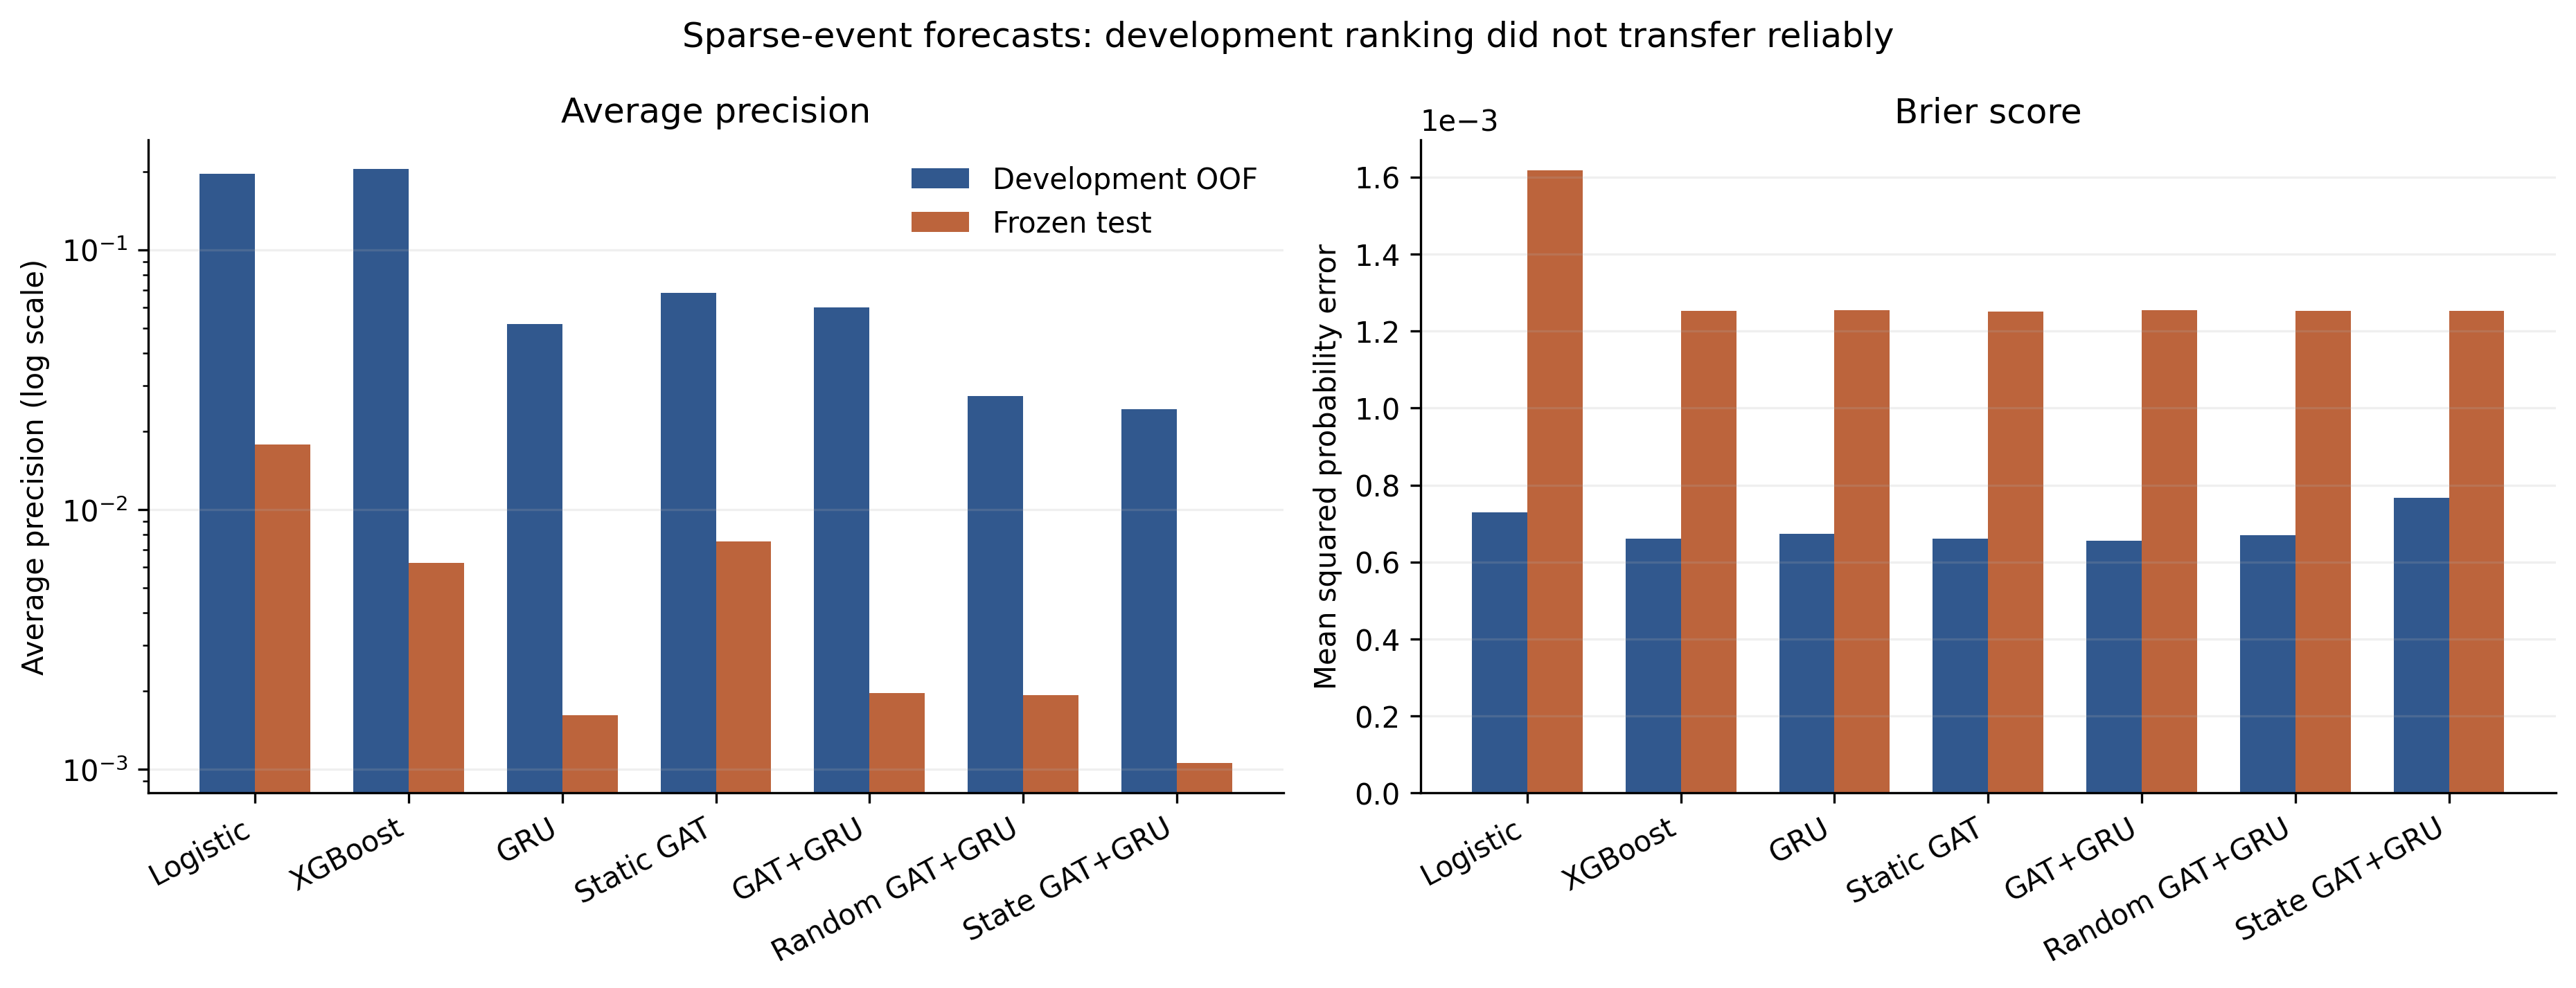
\includegraphics[width=\textwidth]{images/predictive_comparison.png}
\caption{Development OOF and held-out metrics at unchanged settings. Compare Brier within each split: event prevalence differs across periods.}
\end{figure}
\begin{figure}[p]\centering
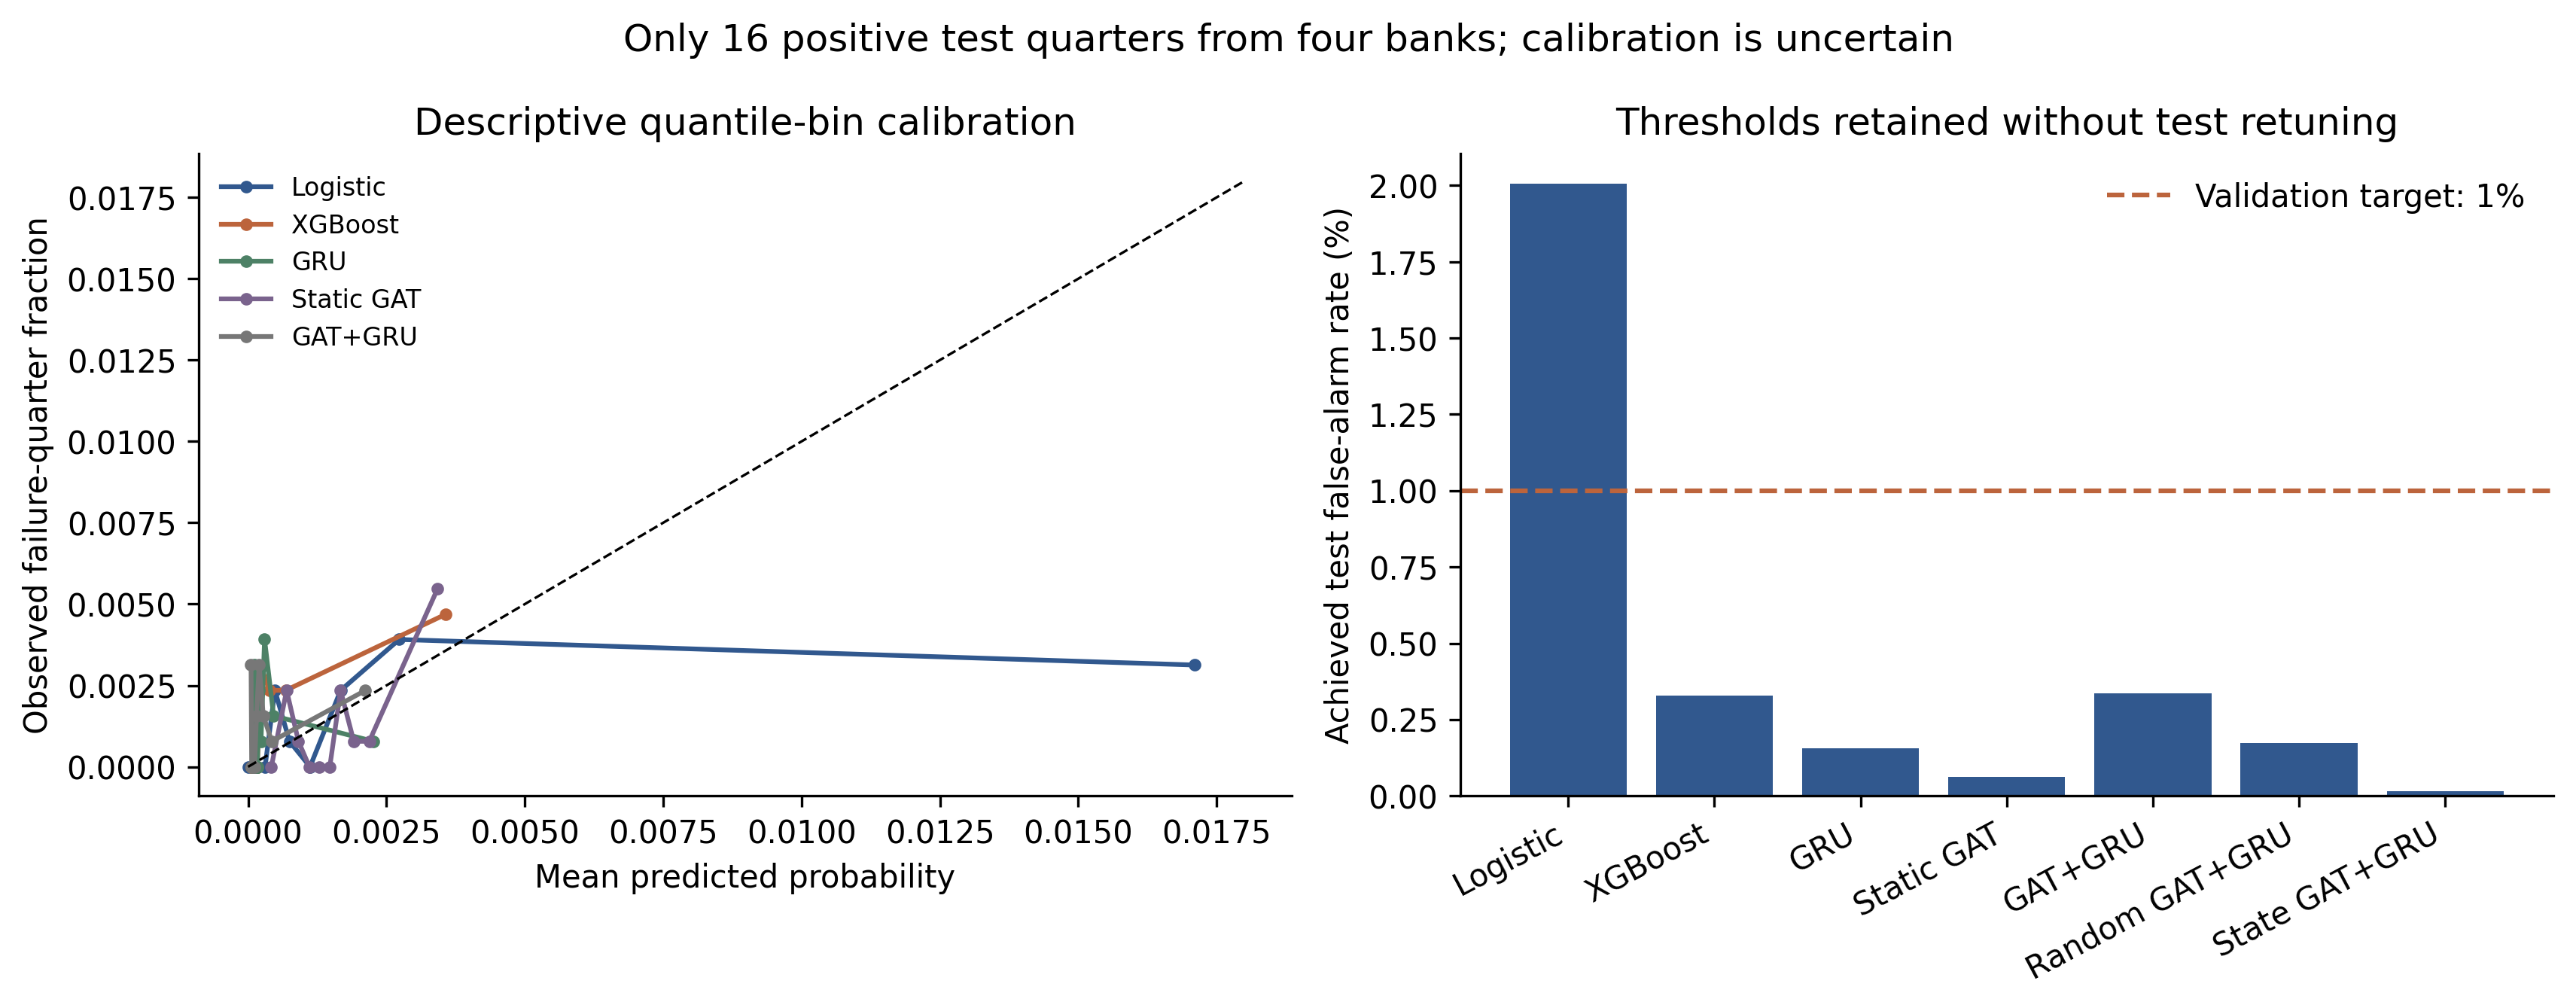
\includegraphics[width=\textwidth]{images/calibration_and_alarms.png}
\caption{Descriptive calibration and achieved test false-alarm rates. The 1\% target was selected on validation, not enforced on test. Sparse positives make calibration uncertain.}
\end{figure}
\begin{figure}[p]\centering
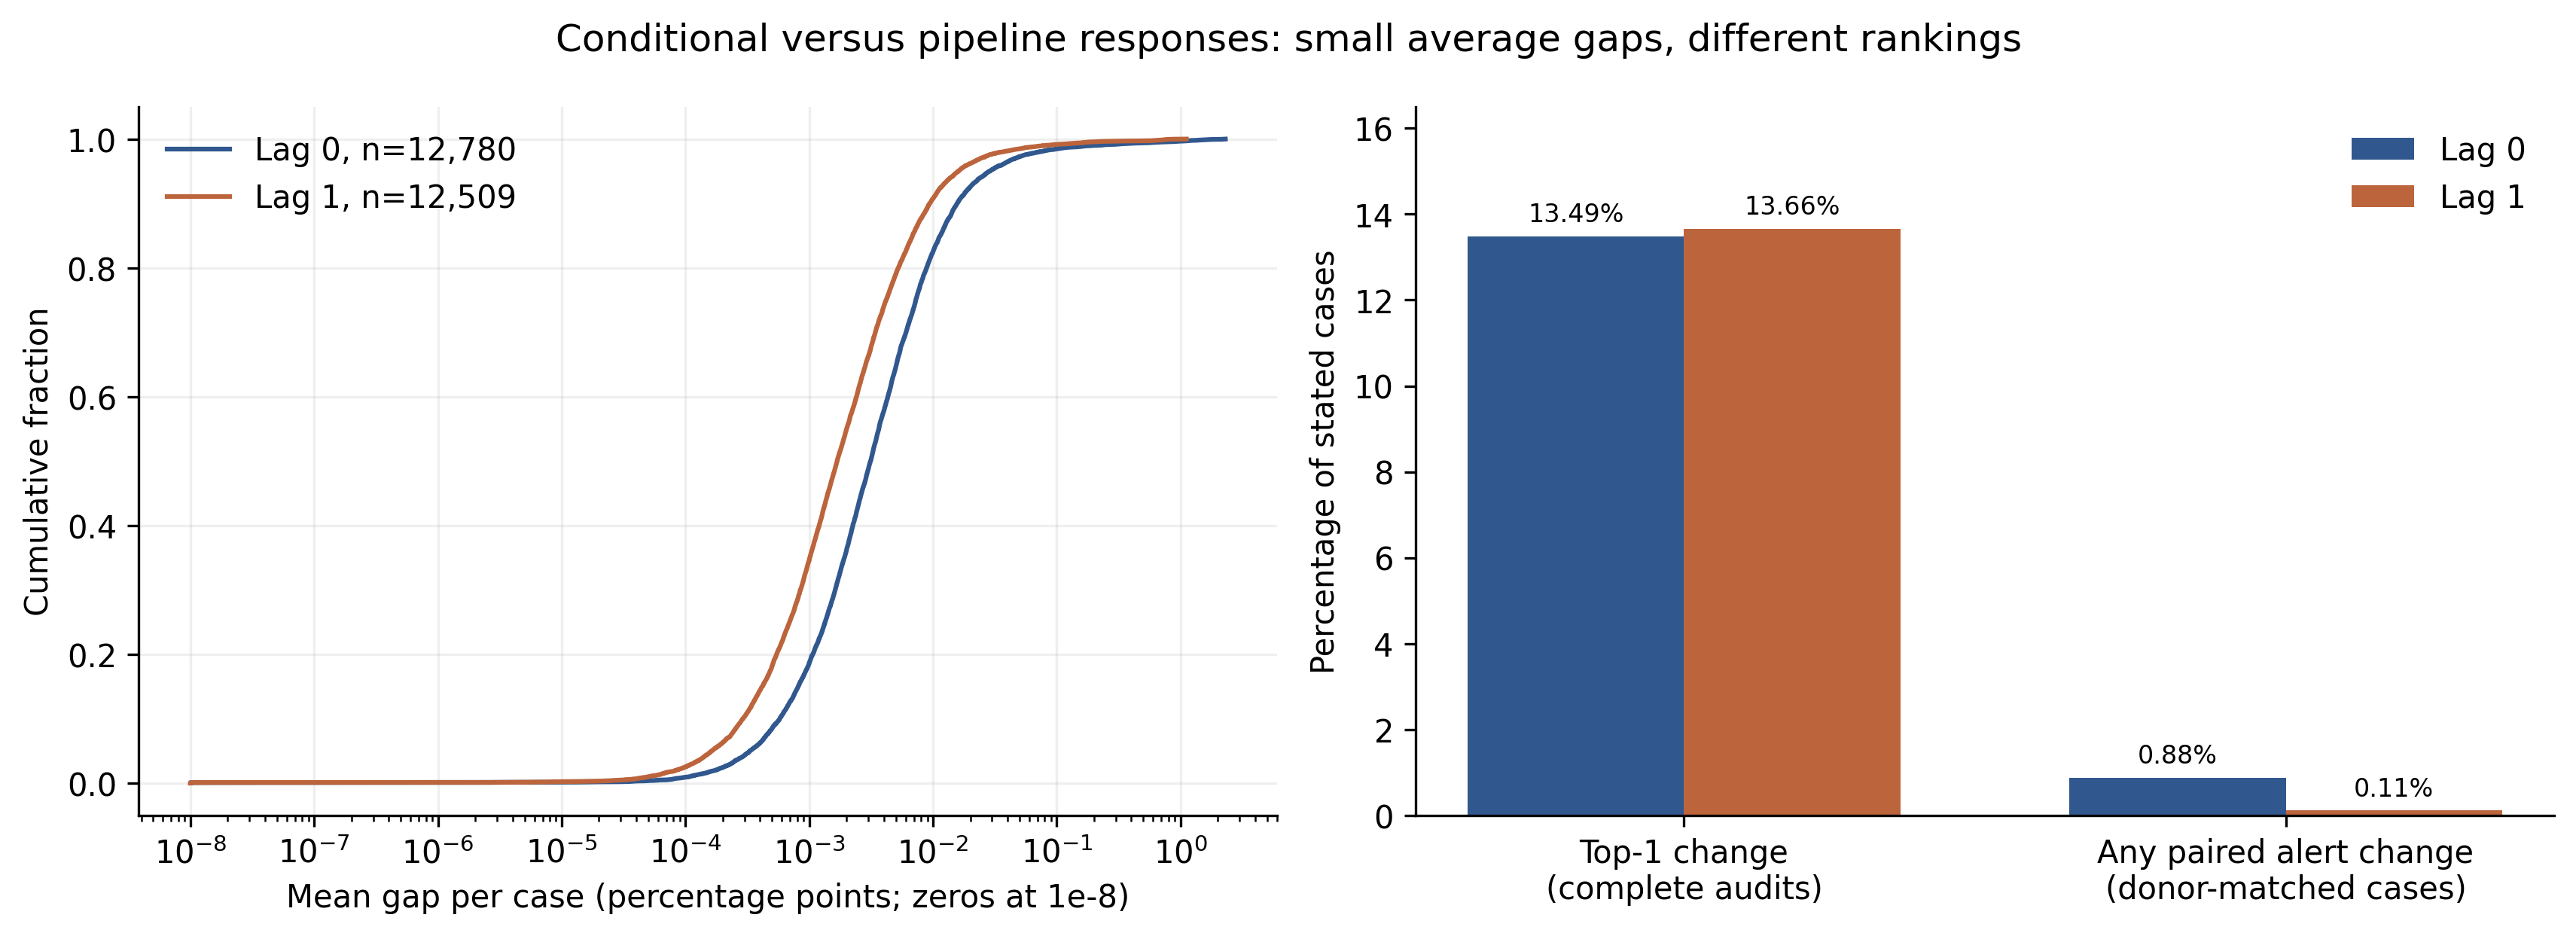
\includegraphics[width=\textwidth]{images/financial_audit.png}
\caption{Primary seed-11 mean-gap distribution and changes in rankings/paired alert decisions. Mean gaps use donor-matched cases; rankings use complete seven-subset cases. Zero gaps use the stated plotting floor.}
\end{figure}
\begin{figure}[p]\centering
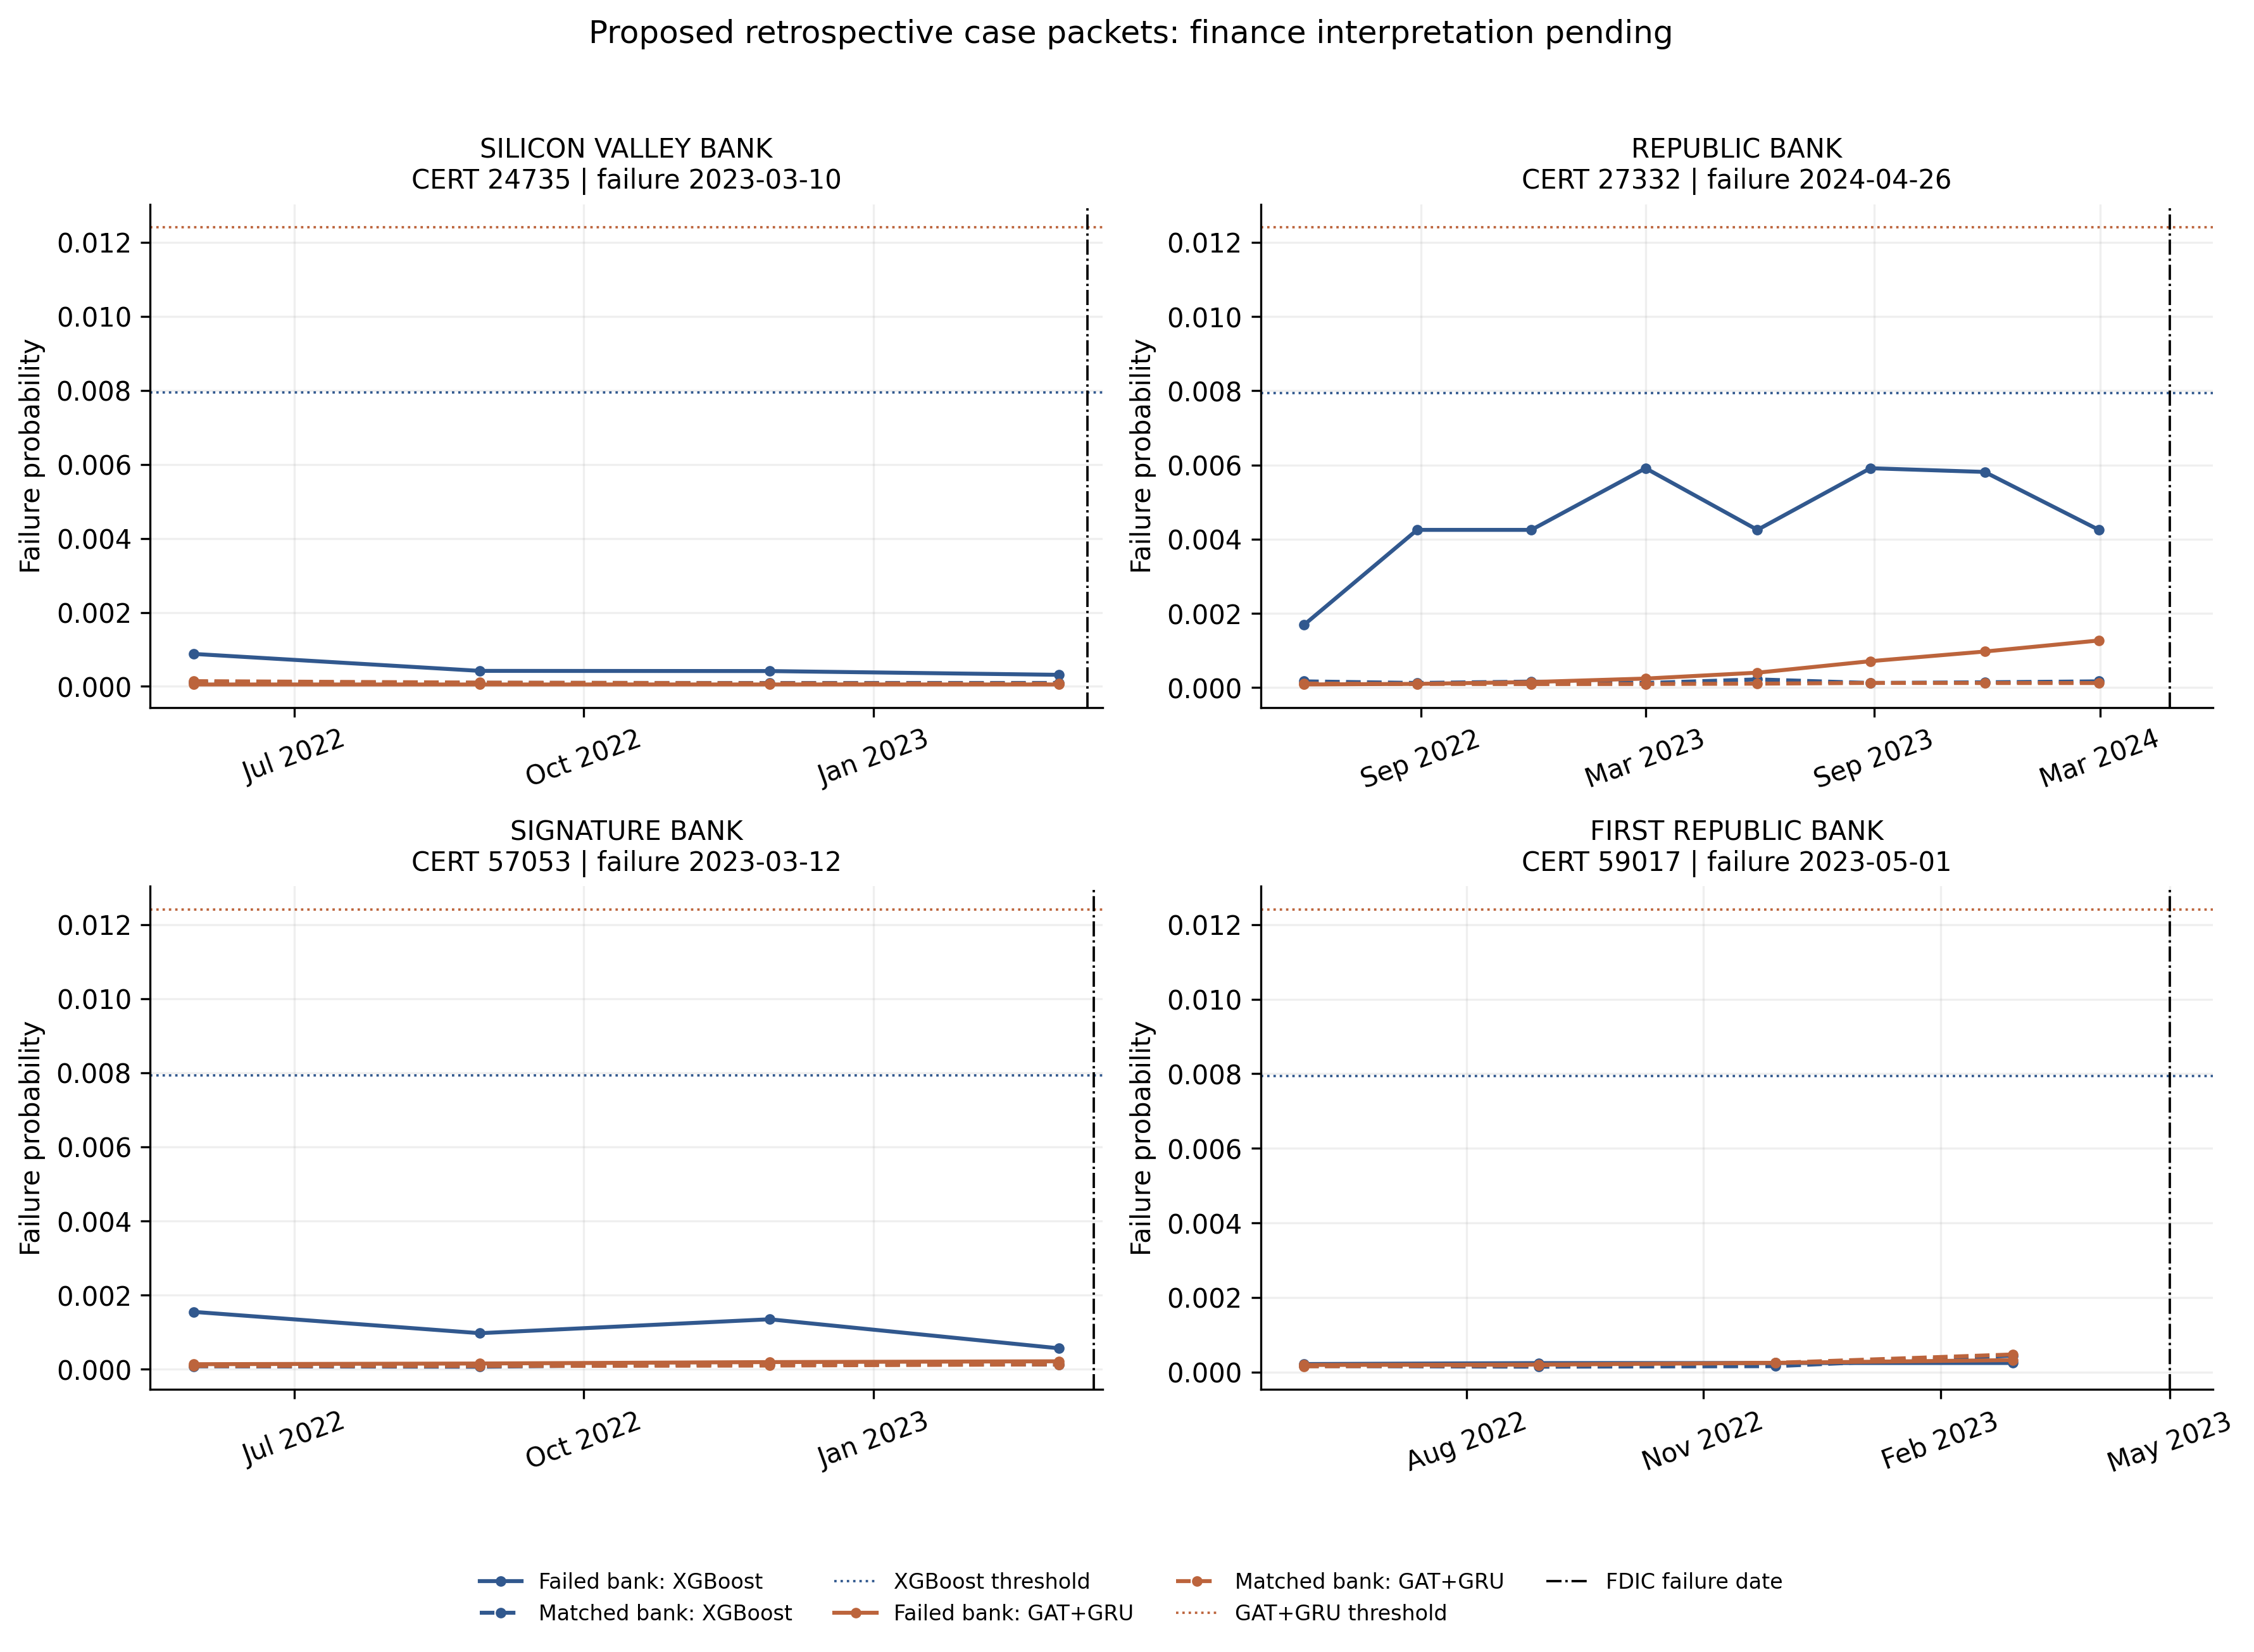
\includegraphics[width=\textwidth]{images/case_forecasts.png}
\caption{Proposed retrospective case packets for the preselected XGBoost and GAT+GRU models. CERT27332 (Republic Bank, 2024) is distinct from CERT59017 (First Republic, 2023). Finance interpretation is pending; these are revised-snapshot reconstructions, not forecasts issued at those dates.}
\end{figure}
\clearpage\bibliographystyle{plainnat}
\bibliography{references}
\end{document}
